\documentclass[utf8]{beamer}

\usepackage[T1]{fontenc}
\usepackage[brazil]{babel}
\usepackage{inconsolata}
\usepackage{minted}
\usepackage[absolute, overlay]{textpos}
\usepackage{graphicx}
\usepackage{changepage} % adjustwidth environment

\definecolor{codebgcolor}{HTML}{FFFFFF}
\definecolor{coderulecolor}{HTML}{5F7FFF}
\definecolor{outerbgcolor}{HTML}{F0F0FF}

\setminted{python3, autogobble,
           breaklines, breakanywhere,
           breaksymbolindentleft=0pt, breaksymbolindentright=0pt,
           breaksymbolsepleft=3pt, breaksymbolsepright=3pt,
           breaksymbolright=...,
           bgcolor=codebgcolor, style=paraiso-light,
           fontsize=\fontsize{8pt}{8pt},
           frame=lines, rulecolor=coderulecolor, framerule=.7pt}
\setmintedinline{bgcolor={}}

\mode<presentation>
\usetheme{Warsaw}
\setbeamercolor{structure}{fg=red!20!black}
\setbeamercolor{background canvas}{bg=outerbgcolor}
\beamertemplatenavigationsymbolsempty

\setbeamertemplate{footline}{\leavevmode\hbox{%
  \begin{beamercolorbox}[wd=.35\paperwidth, ht=2.25ex, dp=1ex, center]
                        {author in head/foot}
    \usebeamerfont{author in head/foot}
      Danilo J. S. Bellini \hfill \texttt{@danilobellini}
  \end{beamercolorbox}%
  \begin{beamercolorbox}[wd=.65\paperwidth, ht=2.25ex, dp=1ex, center]
                        {title in head/foot}
    \usebeamerfont{title in head/foot}
      \insertshorttitle \hfill
      ETEC Uirapuru -- SP \hfill
      \insertshortdate \hfill
      \insertframenumber\,/\,\inserttotalframenumber
  \end{beamercolorbox}%
}}

\title{Segurança da Informação}
\author{Danilo J. S. Bellini \\ \texttt{@danilobellini}}
\date{2018-10-18}

\setlength{\TPHorizModule}{\paperheight}
\setlength{\TPVertModule}{\paperheight}

\renewcommand{\thefootnote}{[\arabic{footnote}]}

\newcommand{\includesvg}[2]{%
  \ifnum\pdfstrcmp{\pdffilemoddate{#2.svg}}%
                  {\pdffilemoddate{#2.pdf}}>0%
    {\immediate\write18%
     {inkscape -z -D --file=#2.svg --export-pdf=#2.pdf --export-latex}%
    }%
  \fi%
  \centering%
  \resizebox{#1}{!}{%
    \input{#2.pdf_tex}%
  }%
}


\begin{document}


\begin{frame}
  \titlepage
  \center Semana de informática \\ ETEC Uirapuru -- SP
  \begin{textblock}{0}(.1, .5)%
    
\includegraphics[height=70pt]{logo-etec-uirapuru.png}%
  \end{textblock}
  \begin{textblock}{0}(.8, .5)%
    
\includegraphics[height=70pt]{banner.png}%
  \end{textblock}
\end{frame}


\begin{frame}{O que é segurança?}
  Estar livre de perigos? Minimizar os riscos?
  \vfill
  Em inglês há duas palavras: safety VS security\footnote{
    Para uma definição mais completa dessas palavras, veja
    \url{http://www.iot.ntnu.no/users/albrecht/rapporter/%
                                notat\%20safety\%20v\%20security.pdf}
  }
  \begin{itemize}
    \item \emph{Safe} refere-se à proteção
          sobre acontecimentos indesejáveis do acaso;
    \item \emph{Secure} refere-se à proteção
          contra acontecimentos intencionais.
          É aqui que se encaixa a segurança da informação.
  \end{itemize}
  \vfill
  Aspectos da segurança da informação:
  \begin{itemize}
    \item Confidencialidade / Privacidade
    \item Integridade
    \item Disponibilidade
  \end{itemize}
  \begin{textblock}{0}(.85, .6)%
    \includesvg{110pt}{Crypto_key}%
  \end{textblock}
\end{frame}


\begin{frame}{Criptografia}
  Criptografia é a prática e o estudo
  das técnicas de armazenamento e comunicação de informação
  na presença de terceiros/adversários.
  \vfill
  Técnicas tradicionais incluem:
  \begin{itemize}
    \item Criptografia de chave simétrica
          (chave única, de conhecimento exclusivo das partes)
    \item Criptografia de chave pública
          (pares de chave pública/privada para cada parte)
    \item Funções de \emph{hash} (sem chave)
  \end{itemize}
  \vfill
  Objetivos:
  \begin{itemize}
    \item \emph{Sign}, assinatura (integridade)
    \item \emph{Encrypt/Decrypt}, encriptação/decriptação
          (confidencialidade)
  \end{itemize}
\end{frame}


\begin{frame}[fragile]{Cifras de César, Vigenère e autochave}
  \begin{columns}[c]
    \column{.6\textwidth}
    Cifra de César (possui 1 parâmetro)
    \resizebox{\textwidth}{!}{%
      \begin{tabular}{rl}
             Mensagem: & \texttt{EU GOSTO DE LIMONADA} \\ \hline
                Chave: & \texttt{C} (desloca 2 no alfabeto) \\
        Texto cifrado: & \texttt{GW IQUVQ FG NKOQPCFC}
      \end{tabular}%
    }
    \vspace{.5em}\vfill
    Cifra de Vigenère (chave simétrica)
    \resizebox{\textwidth}{!}{%
      \begin{tabular}{rl}
             Mensagem: & \texttt{EU GOSTO DE LIMONADA} \\ \hline
                Chave: & \texttt{MENTIRA} \\
        Chave efetiva: & \texttt{ME NTIRA ME NTIRAMEN} \\
        Texto cifrado: & \texttt{QY THAKO PI YBUFNMHN} \\ \hline
                Chave: & \texttt{PAGAZAQ} \\
        Chave efetiva: & \texttt{PA GAZAQ PA GAZAQPAG} \\
        Texto cifrado: & \texttt{TU MORTE SE RILODPDG}
      \end{tabular}
    }
    \vspace{.5em}\vfill
    Autochave (chave simétrica)
    \resizebox{\textwidth}{!}{%
      \begin{tabular}{rl}
             Mensagem: & \texttt{EU GOSTO DE LIMONADA} \\ \hline
                Chave: & \texttt{PAGAZAQP} \\
        Chave efetiva: & \texttt{PA GAZAQ PE UGOSTODE} \\
        Texto cifrado: & \texttt{TU MORTE SI FOAGGOGE}
      \end{tabular}%
    }

    \column{.5\textwidth}
    A cifra de César transforma cada caractere da mensagem
    usando esta tabela:
    \vspace{.5em}\vfill
    \resizebox{\textwidth}{!}{%
      \begin{tabular}{c|c|c|c|c|c}
        \texttt{A} \textrightarrow \texttt{C} &
        \texttt{B} \textrightarrow \texttt{D} &
        \texttt{C} \textrightarrow \texttt{E} &
        \texttt{D} \textrightarrow \texttt{F} &
        \texttt{E} \textrightarrow \texttt{G} &
        \texttt{F} \textrightarrow \texttt{H} \\
        \texttt{G} \textrightarrow \texttt{I} &
        \texttt{H} \textrightarrow \texttt{J} &
        \texttt{I} \textrightarrow \texttt{K} &
        \texttt{J} \textrightarrow \texttt{L} &
        \texttt{K} \textrightarrow \texttt{M} &
        \texttt{L} \textrightarrow \texttt{N} \\
        \texttt{M} \textrightarrow \texttt{O} &
        \texttt{N} \textrightarrow \texttt{P} &
        \texttt{O} \textrightarrow \texttt{Q} &
        \texttt{P} \textrightarrow \texttt{R} &
        \texttt{Q} \textrightarrow \texttt{S} &
        \texttt{R} \textrightarrow \texttt{T} \\
        \texttt{S} \textrightarrow \texttt{U} &
        \texttt{T} \textrightarrow \texttt{V} &
        \texttt{U} \textrightarrow \texttt{W} &
        \texttt{V} \textrightarrow \texttt{X} &
        \texttt{W} \textrightarrow \texttt{Y} &
        \texttt{X} \textrightarrow \texttt{Z} \\
        \texttt{Y} \textrightarrow \texttt{A} &
        \texttt{Z} \textrightarrow \texttt{B}
      \end{tabular}%
    }
    \vfill
    \begin{minted}{python}
      # Código das funções no próximo slide
      msg = "EU GOSTO DE LIMONADA"
      cesar(msg, key="C")
      vigenere(msg, key="MENTIRA")
      vigenere(msg, key="PAGAZAQ")
      autokey(msg, key="PAGAZAQP")
    \end{minted}
    \vfill
    \emph{Desafio}: escrever uma função para cada algoritmo de cifra
                    que encontra o texto original
                    dados a chave e o texto cifrado.
  \end{columns}
\end{frame}


\begin{frame}[fragile]{Cifra de César, Vigenère e autochave em Python}
  \begin{minted}{python}
    from itertools import cycle, accumulate
    from string import ascii_uppercase as alphabet

    def shift_table(key):
        idx = alphabet.find(key)
        return str.maketrans(alphabet, alphabet[idx:] + alphabet[:idx])

    def cesar(msg, key):
        return msg.translate(shift_table(key))

    def vigenere(msg, key):
        parts = msg.split() ; joined = "".join(parts)
        chars = [ch.translate(shift_table(k))
                 for ch, k in zip(joined, cycle(key))]
        positions = accumulate(map(len, parts[:-1]))
        for end in list(positions)[::-1]:
            chars.insert(end, " ")
        return "".join(chars)

    def autokey(msg, key):
        parts = msg.split() ; joined = "".join(parts)
        chars = [ch.translate(shift_table(k))
                 for ch, k in zip(joined, key + joined)]
        positions = accumulate(map(len, parts[:-1]))
        for end in list(positions)[::-1]:
            chars.insert(end, " ")
        return "".join(chars)
  \end{minted}
\end{frame}


\begin{frame}{Chave pública/privada}
  Analogia:
  \begin{adjustwidth}{2em}{1em}\emph{
    Envio pelo correio um cadeado aberto sem a chave,
    o destinatário recebe,
    tranca um pacote com o cadeado e envia p/ mim.
  }\end{adjustwidth}
  Nesse exemplo, o cadeado desempenha o papel de chave pública,
  e a chave do cadeado desempenha o papel de chave privada.
  \vfill
  Vamos ver:
  \begin{itemize}
    \item
    um algoritmo de chave pública/privada
    utilizado para troca de chave simétrica
    \item
    um exemplo prático de uso de chave pública/privada
    no OpenPGP\footnote{
      PGP significa \emph{Pretty Good Privacy},
      um software comercial criado em 1991.
      Sua segunda versão tornou-se o [hoje obsoleto] padrão RFC1991.
      A menos de uma atualização relativa ao algoritmo Camellia,
      RFC4880 (OpenPGP) é a versão mais recente do padrão.
    }.
  \end{itemize}
\end{frame}


\begin{frame}[fragile]{Diffie-Hellman:
                       Exemplo de algoritmo para troca de chave}
  \begin{columns}[c]
    \column{.5\textwidth}
    \includesvg{\textwidth}{Diffie-Hellman_Key_Exchange}

    \column{.5\textwidth}
    \resizebox{\textwidth}{!}{%
      \begin{tabular}{rl}
        Número primo (público): & $p$ \\
        Base (público): & $g$ \\
        Chave privada da Alice: & $a$ \\
        Chave pública da Alice: & $A = g^a \mod p$ \\
        Chave privada do Bob: & $b$ \\
        Chave pública do Bob: & $B = g^b \mod p$ \\
        Número compartilhado: & $A^b \equiv B^a \mod p$
      \end{tabular}%
    }
    \vspace{.5em}\vfill
    Exemplo:
    \begin{minted}{python}
      # Alice e Bob combinam os parâmetros
      p = 2551
      g = 2

      # Criam chaves privadas em silêncio
      a = 45
      b = 29

      # Calculam e trocam chaves públicas
      A = (g ** a) % p          # 2285
      B = (g ** b) % p          # 207

      # Alice e Bob possuem um segredo!
      secret = (A ** b) % p     # 414
      secret = (B ** a) % p     # 414
    \end{minted}
  \end{columns}
\end{frame}


\begin{frame}[fragile]{GPG~-- \emph{GNU Privacy Guard}}
  O GPG é uma implementação em software livre (GPLv3)
  que atende ao OpenPGP (maiores detalhes no próximo slide)
  sem utilizar softwares/algoritmos patenteados/restritos/privados.
  \begin{minted}{shell}
    gpg --gen-key # Criar chaves (par público/privado)
    gpg -k        # Visualizar chaves disponíveis

    # Exportando/importanto chaves públicas (para um dado keyID)
    gpg --keyserver pgp.mit.edu --send-keys keyID
    gpg --keyserver pgp.mit.edu --recv-keys keyID
    gpg --export --armor danilo.bellini@gmail.com > my.key
    gpg --import my.key

    # Assinatura
    gpg -b message.txt                       # Assina (cria ".sig")
    gpg --verify message.txt.sig message.txt # Verifica assinatura

    # Codificando/criptografando (crypt) p/ um destinatário específico
    gpg -o encrypted.gpg -r danilo.bellini@gmail.com -e message.txt

    # Decodificando/decriptografando (decrypt) com a chave privada
    gpg -o decrypted.txt -d encrypted.gpg

    # Comandos utilizados na apresentação (além de vim, cat, rm, ...)
    seq 15 > message.txt     # Cria message.txt c/ sequência de 1 a 15
    hexdump -C encrypted.gpg # Visualizando arquivos como binários
  \end{minted}
\end{frame}


\begin{frame}[fragile]{Tomb: armazenamento criptografado em um arquivo}
  Discos rígidos, SSDs, SDs e outras mídias
  normalmente não estão criptografados.
  \emph{Tomb} permite criarmos diretórios criptografados
  com uma chave criptografada com GPG escondida em uma imagem.
  \vfill
  \begin{minted}{shell}
    tomb dig new.tomb -s 50          # Cria o new.tomb com 50MB
    tomb forge new.key -g            # Cria uma chave encriptada com GPG
    tomb lock new.tomb -k new.key -g # Atribui a chave e formata o new.tomb

    tomb open new.tomb -k new.key -g # Monta o new como se fosse um pendrive
    tomb close new                   # Desmonta o new

    # Esteganografia
    cp EnigmaMachine.jpg new.jpg     # Cópia para não perder a imagem original
    tomb bury new.jpg -k new.key -g  # Armazena chave (+ senha) na imagem
    tomb exhume new.jpg -k copy.key  # Extrai a chave da imagem
    tomb open new.tomb -k new.jpg -g # Podemos usar a imagem direto
  \end{minted}
  \vfill
  \begin{columns}[c]
    \column{.15\textwidth}
    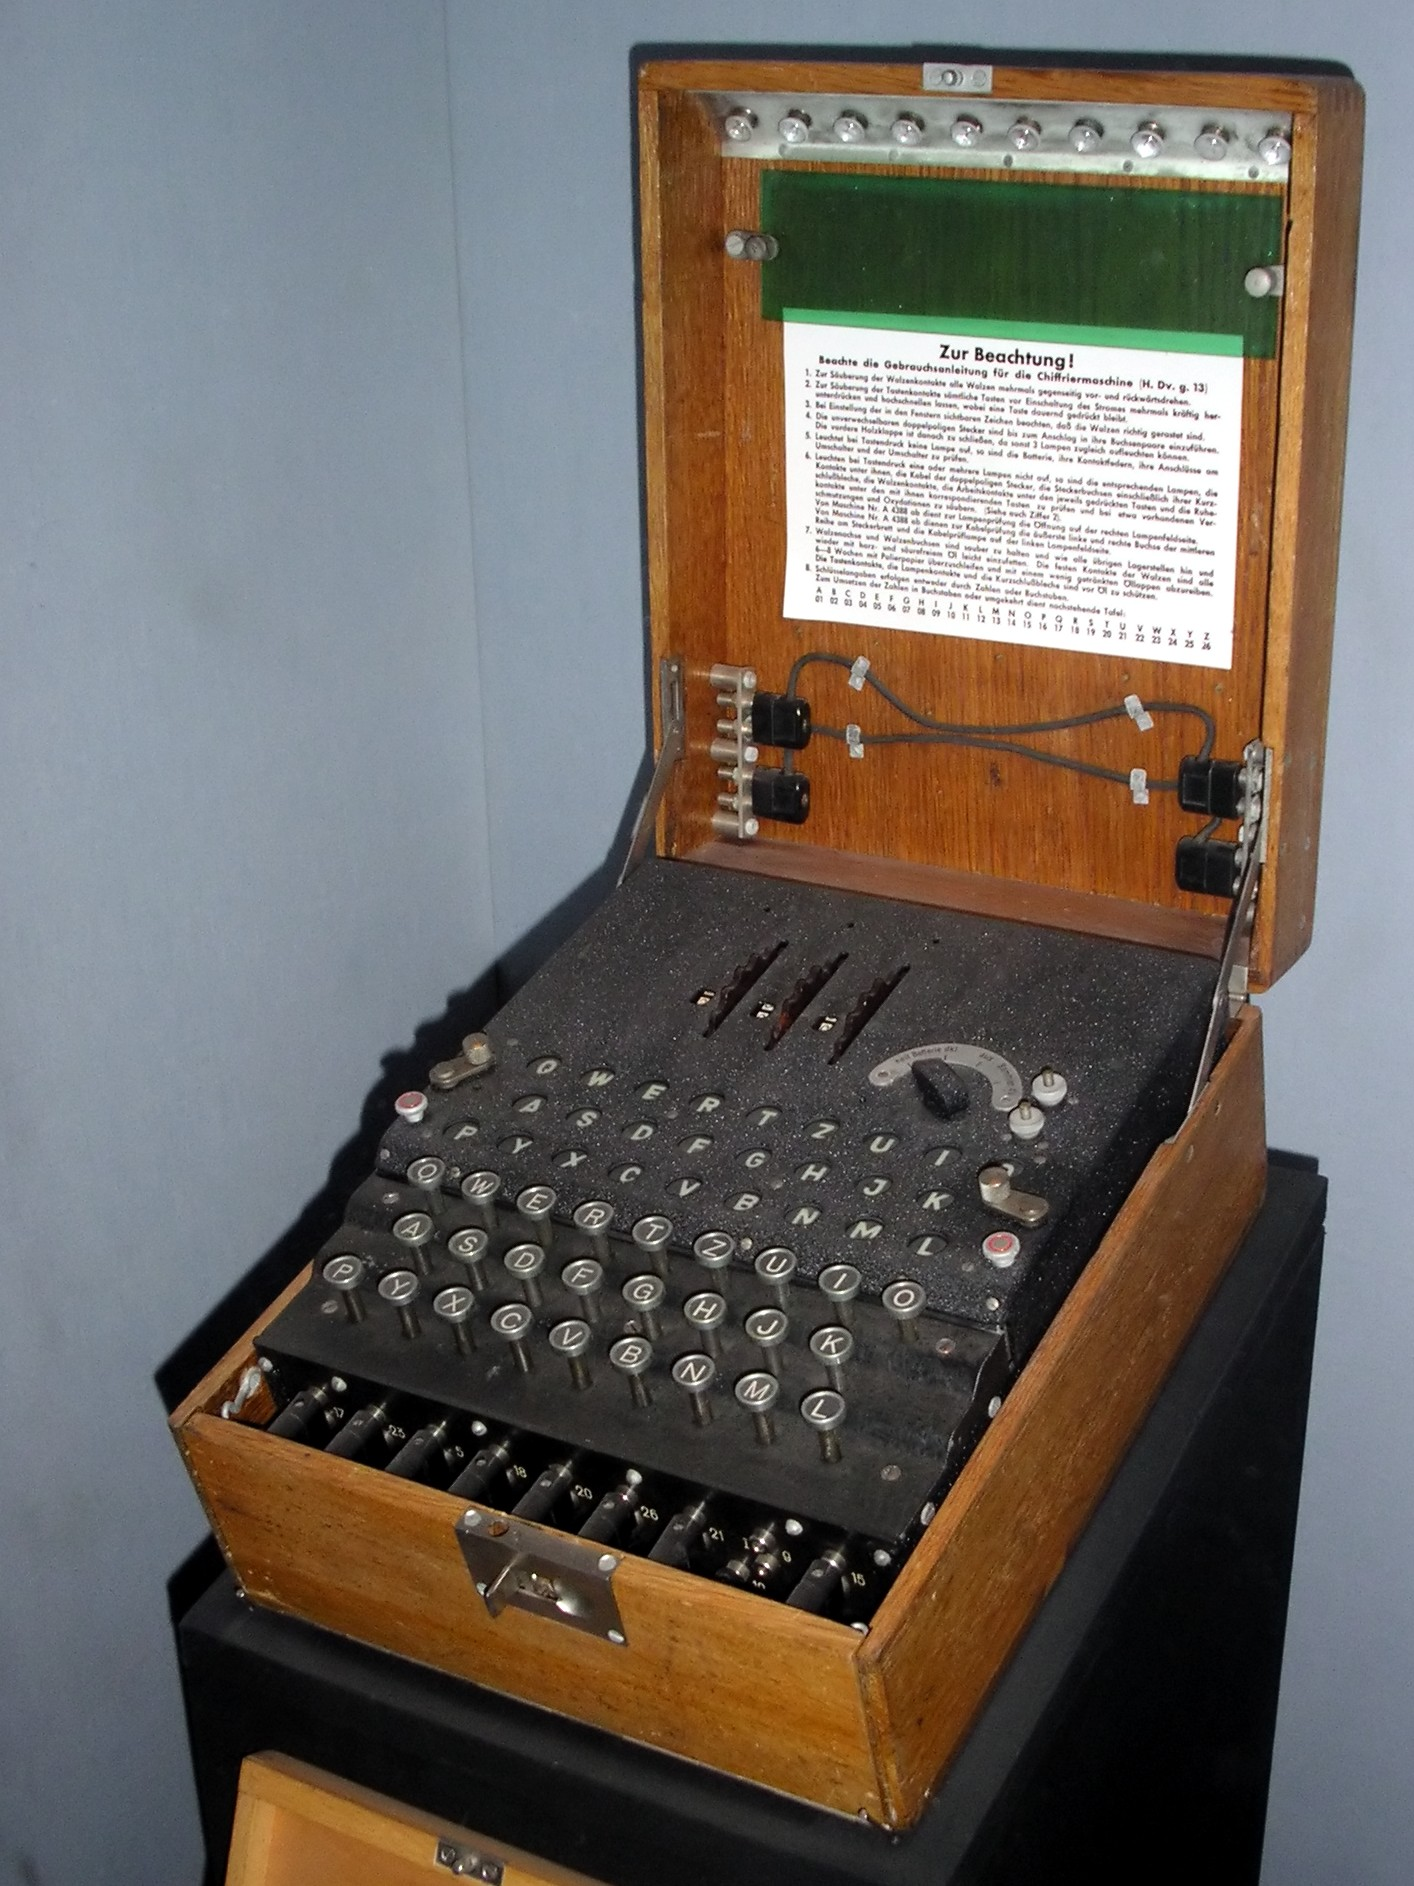
\includegraphics[height=60pt]{EnigmaMachine.jpg}
    \column{.85\textwidth}
    \centering
    Quem imaginaria que a imagem ao lado poderia conter uma chave?
    \vfill
    Use senhas fortes (mais sobre isso em breve)!
  \end{columns}
\end{frame}


\begin{frame}
  \centering
  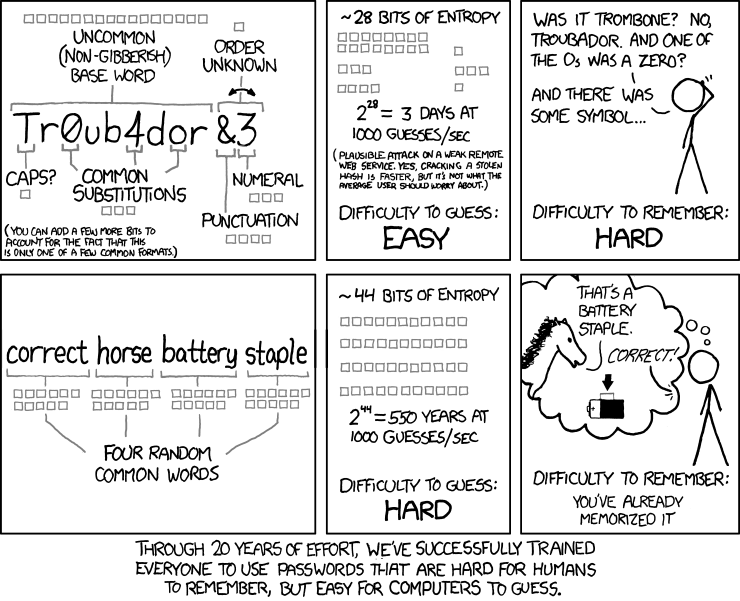
\includegraphics[width=.8\textwidth]{password_strength.png}
  \url{https://www.xkcd.com/936/}
  \vfill
  São $\approx 44$ bits se considerarmos mensagens de $4$ palavras
   em um universo de $2000$ palavras equiprováveis
\end{frame}


\begin{frame}
  \begin{columns}[c]
    \column{.5\textwidth}
    \centering
    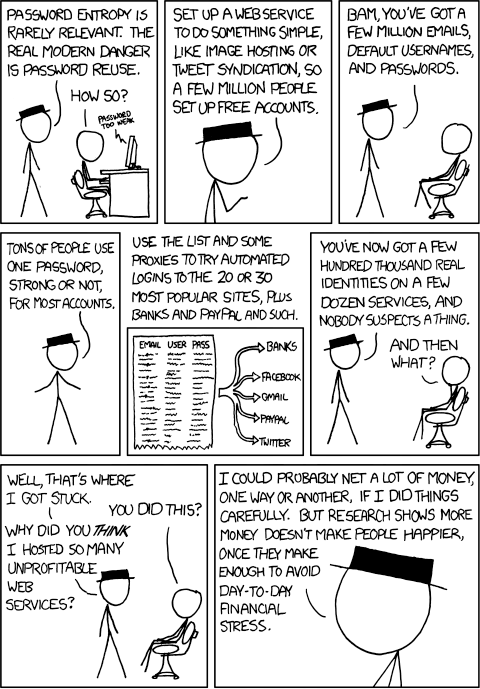
\includegraphics[width=\textwidth]{password_reuse_1.png}
    \column{.5\textwidth}
    \centering
    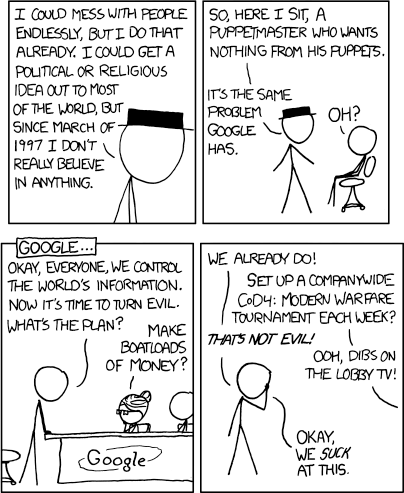
\includegraphics[width=\textwidth]{password_reuse_2.png}
    \url{https://www.xkcd.com/792/}
  \end{columns}
\end{frame}


\begin{frame}
  \centering
  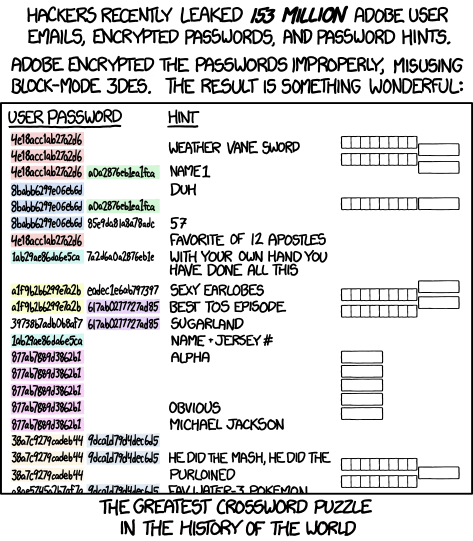
\includegraphics[width=.7\textwidth]{encryptic.png}
  \url{https://www.xkcd.com/1286/}
\end{frame}


\begin{frame}{Referências}
  O material abaixo está disponível apenas em inglês.
  \begin{itemize}
    \item Livro de GPG:
          \url{https://www.gnupg.org/gph/en/manual/book1.html}
    \item Tutorial de GPG:
          \url{https://www.futureboy.us/pgp.html}
    \item Página oficial do Tomb:
          \url{https://www.dyne.org/software/tomb/}
    \item Resumo sobre o Tomb:
          \url{https://pujol.io/blog/tomb-with-gpg-keys/}
    \item RFC1991 (PGP, obsoleto):
          \url{https://tools.ietf.org/html/rfc1991}
    \item RFC4880 (OpenPGP):
          \url{https://tools.ietf.org/html/rfc4880}
  \end{itemize}
  Todas as imagens utilizadas nos slides sem fonte explícita
  foram obtidas do Wikipedia,
  exceto as do slide inicial,
  as quais foram obtidas em \url{http://etecuirapuru.com.br/}.
\end{frame}


\begin{frame}
  \begin{center}\fontsize{5cm}{2.5cm}\selectfont
    FIM!
  \end{center}
\end{frame}


\end{document}
